\documentclass[10pt,a4paper]{article}

\sloppy
\usepackage{caption}
\usepackage{subcaption}
\captionsetup[subfigure]{justification=centering}
\captionsetup{font = footnotesize, labelfont = bf}
\captionsetup[sub]{font=scriptsize,labelfont= bf, justification = centering, margin = 0cm}

\setlength{\textwidth}{16cm}
\setlength{\textheight}{23cm}
\addtolength{\hoffset}{-1.5cm}
\addtolength{\voffset}{-1.5cm}
\setlength{\headheight}{35pt}
\usepackage[utf8]{inputenc}
%\usepackage[spanish]{babel}
\usepackage[spanish,es-tabla]{babel}
\usepackage{ae}
\usepackage{graphicx}
\usepackage{wrapfig}
\usepackage{tikz,pgfplots}
\usepackage{epsfig}
%\usepackage{multicol, array}
\usepackage{amsmath}
\usepackage{amssymb, amsthm}
\usepackage{amsfonts}
\numberwithin{equation}{section}% reset equation counter for sections
\numberwithin{equation}{subsection}


\DeclareMathOperator\erf{erf}
\usepackage{euscript}
\usepackage{mathrsfs}
\usepackage{sectsty}
\usepackage{lipsum}
\usepackage{courier}
\usepackage{listings}
\usepackage{xcolor}
\definecolor{verde}{rgb}{0.0, 0.5, 0.1}

\lstset{
  language=R, literate =  {á}{{\'a}}1 {é}{{\'e}}1 {í}{{\'{\i}}}1 {ó}{{\'o}}1 {ú}{{\'u}}1 {Á}{{\'A}}1 {É}{{\'E}}1 {Í}{{\'I}}1 {Ó}{{\'O}}1 {Ú}{{\'U}}1 {ü}{{\"u}}1 {Ü}{{\"U}}1 {ñ}{{\~n}}1 {Ñ}{{\~N}}1,
  backgroundcolor=\color{gray!6!},
  classoffset=0,
  basicstyle=\ttfamily\small\bfseries,
  showspaces=false,
  showstringspaces=false,
  keywordstyle=\color{blue!60!black}\bfseries,
  stringstyle=\color{blue},
  numbers=none,
  numberstyle=\ttfamily\small,
  commentstyle=\color{verde}\textbf,
  morecomment=[l][\color{verde}\textbf],
  frame = single,
  framexleftmargin= -0pt,
  framexrightmargin= -5pt}


\usepackage{tcolorbox}
\tcbuselibrary{theorems}

\newtcbtheorem[auto counter,number within=section]{theorem}{Teorema}%
{colback=green!5,colframe=green!35!black,fonttitle=\bfseries}{th}

\newtcbtheorem[auto counter,number within=section]{definition}{Definición}%
{colback=blue!5,colframe=blue!35!black,fonttitle=\bfseries}{def}

\newtcbtheorem[auto counter,number within=section]{example}{Ejemplo}%
{colback=red!5,colframe=red!35!black,fonttitle=\bfseries}{ej}


%\newtcbtheorem[auto counter,number within=section]{theorem}{Teorema}%
%{colback=green!5,colframe=green!35!black,fonttitle=\bfseries}{th}

\newtcbtheorem[auto counter,number within=section]{software}{Software}%
{colback=yellow!5,colframe=yellow!35!black,fonttitle=\bfseries}{sw}

\usepackage{fancyhdr}

\decimalpoint
\usepackage[T1]{fontenc}
%\usepackage{textcomp}

\pagestyle{fancy}
\lhead{U.N.S.L. - Departamento de Física\\Lic. en Física - Física Experimental I}
\rhead{
\includegraphics[width=0.8cm]{unsl.jpg}}
\pagenumbering{arabic}
%\rhead{
\includegraphics[width=0.80cm]{unsl.jpg}}

%\setcounter{page}{1}
\setlength{\parskip}{3mm}

\pgfplotsset{compat=1.13}

\usepackage{hyperref}
\hypersetup{
    colorlinks=true,
    linkcolor=blue,
    filecolor=black,      
    urlcolor=blue,
    citecolor=black,
   	anchorcolor=black
}
 
\urlstyle{same}
\usepackage{lettrine}
\setcounter{DefaultLines}{4}
% \renewcommand{\tablename}{Tabla}
\begin{document}

\begin{center}
{
\begin{large}
\textbf{Laboratorio N$^o$ 2:} \\
\vspace*{0.1cm}
 \textbf{Concepto de Medida e Incertezas Asociadas, v.2}
\end{large}
}
\end{center}

\section*{Introducción}

En este laboratorio vamos a discutir algunas cosas relacionadas a uno de los sistemas físicos que van a estudiar a lo largo de toda la carrera: el péndulo. Vamos a tocar tres ideas:

\begin{itemize}
\item[$\bullet$] \textit{Modelado}: Péndulo \textit{ideal}.
\item[$\bullet$] \textit{Modelo de sistema físico}: vamos a ver que un rudimento de cómo intentar \textit{corroborar} un modelo.
\item[$\bullet$] \textit{Incertezas}: Idea de media muestral, desviación estándar de la muestra y error estándar de la media.
\item[$\bullet$] \textit{Errores sistemáticos}: Vamos a buscar por errores sitemáticos en caso de que nuestro modelo no se corrobore.
\end{itemize}

\section{Péndulo Ideal}

\subsection{Introducción: Modelo}

\begin{wrapfigure}{l}{0.3\textheight} 
%\centering
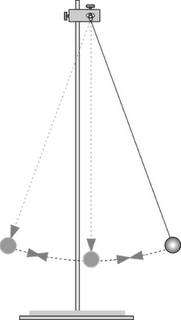
\includegraphics[width=0.3\textwidth]{./graf/pendulo.png}
\vspace{0mm}  
\caption{Esquema de péndulo.} 
\label{pendulo}  
\vspace{-17mm}
\end{wrapfigure}

Un péndulo ideal consiste en una \textit{masa puntual} $m$ colgada de un hilo \textit{idealmente} inelástico y sin masa, que se mueve --idealmente-- sin fricción alguna, \textit{oscilando} indefinidamente luego de ser sacado del estado de equilibrio. Un esquema del péndulo ideal se muestra en la Fig.(\ref{pendulo}).

Decimos que el periodo $\tau [s]$ de un péndulo es el intervalo de tiempo que el péndulo demora en completar un ciclo de movimiento. 
Se sabe que el periodo de un péndulo $\tau[s]$ está dado, cuando las oscilaciones son \textit{pequeñas}, por:
\begin{equation} \label{tau}
\tau = 2\pi \sqrt{l/g}
\end{equation} 
\noindent donde $l[m]$ es la longitud en la cual el péndulo oscila, y $g[m/s^2]=9.80m/s^2$ es la aceleración de la gravedad. Es importante notar que, según este modelo, el periodo del péndulo:
\begin{itemize}
\item[$\bullet$] No depende de la masa del péndulo.
\item[$\bullet$] No depende de la amplitud de oscilación (el valor máximo del ángulo de oscilación).
\item[$\bullet$] Cambia sólo con el largo $l$ del hilo. 
\end{itemize}

\vspace{5mm}

En la Fig.\eqref{glineal} se muestra $\tau$ \textit{vs.} el largo del péndulo $l$; es posible observar que el periodo crece en función de la raíz cuadrada del largo del péndulo, $\sqrt{l}$.

\begin{figure}[h!]
\centering
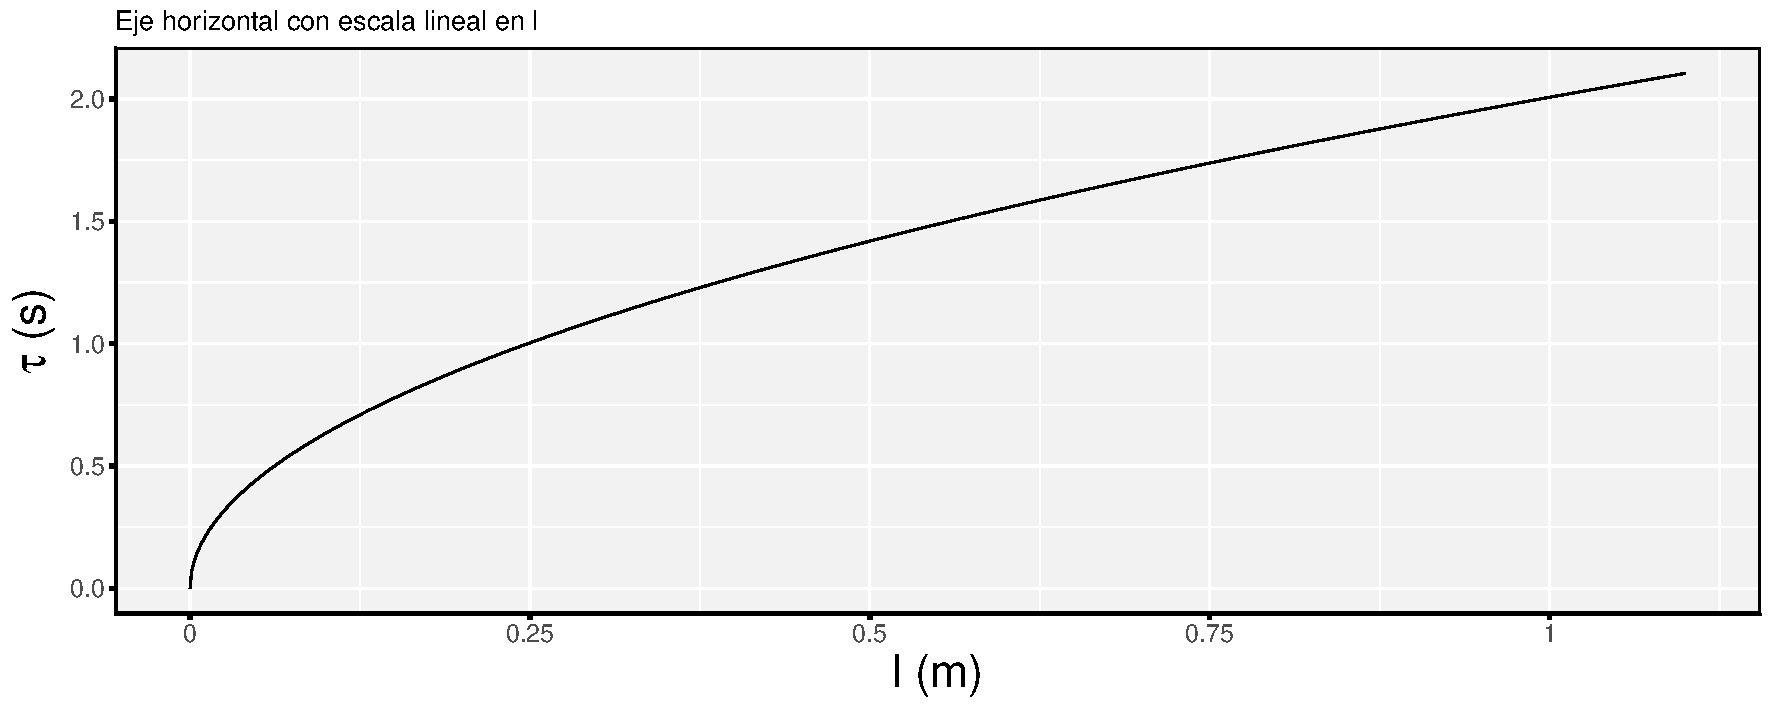
\includegraphics[width=1\linewidth]{./graf/graflineal.pdf}
\vspace*{-2.5mm}
\caption{Gráfica del periodo $\tau \, [s]$ \textit{vs.} el largo $l \, [m]$.}  
\label{glineal}
\vspace*{0mm}  
\end{figure}


El péndulo es uno de los sistemas físicos más utilizados para modelar otros sistemas (es un \textit{toy model}\footnote{\textit{Toy Model}, literalmente, \textit{modelo de juguete}: un sistema simple que permite explicar a \textit{grosso modo} ciertas características de otros sistemas.} muy popular en la física). Lo usaremos hoy y lo seguiremos usando a lo largo del curso. No hace falta que comprendan la física del péndulo (por ahora), aunque es un sistema estudiado en todos los cursos de mecánica.

En este laboratorio, nos proponemos corroborar la ec.\eqref{tau} para \textbf{(a)} un valor de $\tau$ y un valor de $l$ particular (cada estudiante hará una experiencia); \textbf{(b)} la colección de $\{l_i, \tau_i\}$ de todo el curso. 

\subsection{Montando un péndulo real...¿o era ideal?}
Tiempo de experiencia: 45 minutos

\begin{wrapfigure}{r}{0.5\linewidth}
\vspace*{-8mm}
\begin{center}
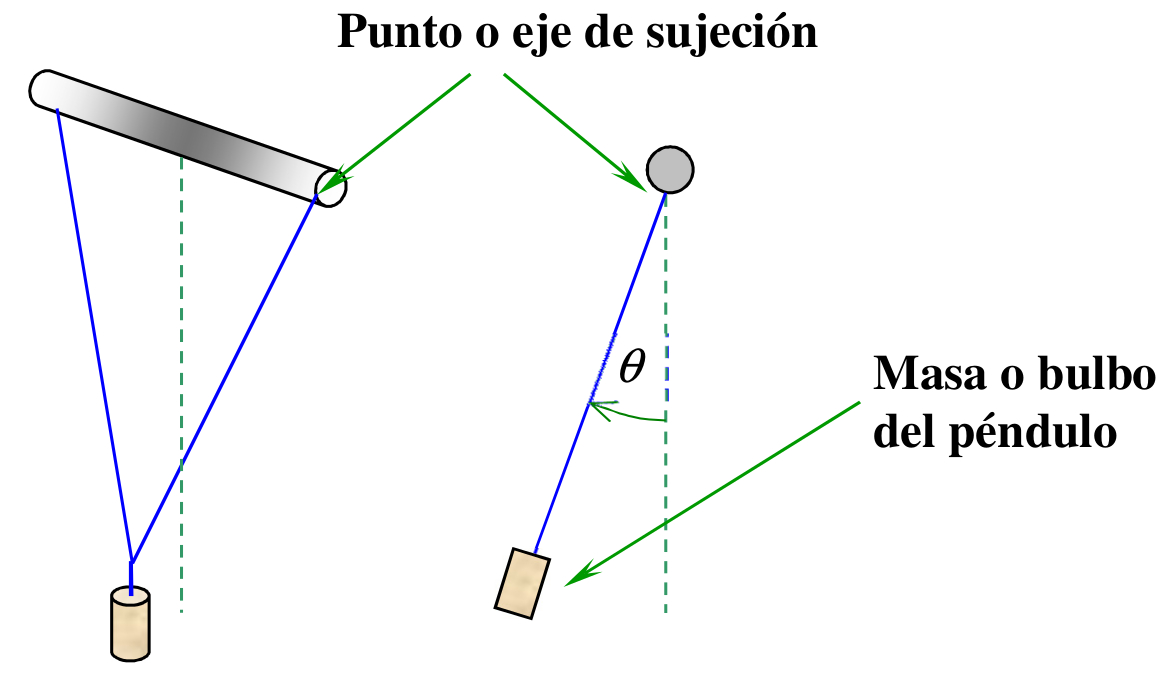
\includegraphics[width=1\linewidth]{./graf/pendulogil.jpg}
\vspace*{-2mm}
\caption{Esquema para mostrar la configuración \textit{bifilar} utilizada. Esta configuración permite obtener oscilaciones en un plano.}
\label{gpconf}
\end{center}
\vspace*{-8mm}
\end{wrapfigure}

Una de las posibilidades para montar un péndulo es la conocida configuración \textit{bifilar}, que se muestra en la Fig.\eqref{gpconf}. Esta configuración permitirá obtener oscilaciones en un plano, que luego facilitarán la medida que realizaremos (que será con un cronómetro). Para el \textit{hilo inextensible y sin masa}, utilizaremos hilo de coser. Para la \textit{partícula puntual} de masa $m$ tendremos que utilizar algún objeto de \textit{dimensiones finitas}, al que llamaremos \textit{masa} o \textit{bulbo} (Fig.\eqref{gpconf}).

Estas modificaciones respecto de nuestro modelo ideal deben ser consideradas en la práctica experimental: tanto la masa del hilo como la finitud del objeto imponen modificaciones que debemos tener en cuenta a la hora de realizar medidas. Si la masa del hilo no es cero, debe ser \textit{despreciable} respecto de la masa del bulbo. Si el bulbo no es un punto, deben ser tenidas en cuenta las dimensiones y la geometría del objeto.

Para el caso de la masa del hilo, baste decir que debe representar menos del $1\%$ de la masa del bulbo. En cuanto a las dimensiones y la geometría del bulbo, diremos que la distancia $l$ puede ser considerada como la distancia desde el eje de rotación o sujeción hasta el \textit{centro de masa} del bulbo.

Mientras que la masa del hilo es fácilmente \textit{cuantificable}, el centro de masa puede representar algún problema. En principio, debemos tener en cuenta que, asumiendo que el bulbo tiene \textit{densidad} constante, obtendremos que el centro de masa coincidirá con el \href{https://es.wikipedia.org/wiki/Centroide}{centroide} del bulbo. En tal caso, mediremos la distancia desde el eje de rotación hasta la posición vertical del centroide. 

Una práctica común en la experimentación --y en la teoría y en la vida cotidiana y en \textit{etc}...-- consiste en planear criterios de validación sobre las suposiciones que se realizan...como la asunción de densidad constante. Es por esto que propondremos un par de medidas extra de longitud, para obtener cotas de la posible posición del centro de masa.

\section{Actividad: ¿El modelo funciona para el par de valores ${l, \tau}$?}


\noindent \begin{footnotesize} \textbf{Nota:} cada estudiante construirá un péndulo mediante el empleo de una masa (puede ser el cilindro empleado en la experiencia anterior) y un hilo, provisto por la cátedra. La longitud del péndulo será asignada a cada estudiante por la cátedra.\end{footnotesize}



La idea básica será corroborar la ec.\eqref{tau} para \textit{un par de valores de la ecuación} $\{l,\tau\}$. Esta no es una corroboración \textit{muy coqueta} (luego veremos más), pero \textit{peor es nada}. Para pensar en la corroboración del modelo, tenemos que:

\begin{equation}
\tau = 2\pi \sqrt{\frac{l}{g}} \overbrace{\quad \Longrightarrow \quad}^{\text{Midiendo } \tau \text{ y } l \text{ obtenemos}}
\begin{cases}
\text{una colección de valores de } \tau_i \text{ con } i = 1,2,3,...,n\\
\text{un valor de } l \pm \delta l \text{ y luego } \tau_{Modelo} = 2 \pi \sqrt{l/g}\\
\end{cases}
\end{equation}


Una vez que tengamos ${l, \tau_i}$ medidos, podemos despejar la gravedad de la ec.(\eqref{tau}), obteniendo: 
\begin{equation}\label{etaumodelo}
g_{Modelo} = 4 \pi^2 \frac{l}{\tau^2}
\end{equation}

\noindent puesta en esta forma, vamos a usar el valor de referencia de $g [m \, s^{-2}]$ de la \href{https://www.ign.gob.ar/NuestrasActividades/Geodesia/Gravimetria/RAGA}{Red Argentina de Gravedad Absoluta}\footnote{Es posible descargar la planilla de datos y buscar el punto medido en La Florida, San Luis. Según la Dra. Silvana Spagnotto (geofísica), la medida en el Embalse La Florida es mayor en $5  \; mgal$ respecto de la Ciudad de San Luis.}.

Es claro que, como tendremos resultados experimentales, la igualdad en la ec.\eqref{tau} está \textit{matizada}, debido a que las magnitudes con las que trataremos tendrán incertezas.
\pagebreak

\section{Midiendo}

\subsection*{Midiendo el largo del péndulo}
\begin{wrapfigure}{r}{0.15\linewidth}
\vspace*{-17.5mm}
\begin{center}
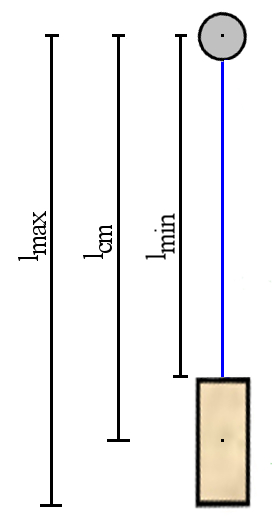
\includegraphics[width=1\linewidth]{./graf/medidasl.jpg}
\vspace*{-7.5mm}
\caption{Las distancias a medir, $l_{min}$, $l_{cm}$ y $l_{max}$}
\label{gmedidas}
\end{center}
\vspace*{-8mm}
\end{wrapfigure}

Ya anticipamos que la medida del largo del péndulo puede presentar problemas, pues el modelo del que disponemos, explicita que $l$ es la distancia entre el eje de sujeción y una partícula puntual de masa $m$. Una posible solución --ya nombrada-- es considerar el bulbo como un objeto de densidad constante e identificar centroide con el centro de masa\footnote{¿Y el centro de masa con el centro de gravedad?}.

Como un elemento de juicio \textit{extra}, que nos servirá para corroborar la afirmación, será --además de medir la distancia perpendicular desde el eje de sujeción al centroide-- medir las distancias perpendiculares mínima y máxima al objeto. Esto nos dará material de análisis posterior, ya que tendremos algún elemento de juicio extra sobre las cotas en las que puede encontrarse el centro de masa.


Un esquema de las distancias a medir puede ser observado en la Fig.\eqref{gmedidas}, donde se muestran $l_{min}, l_{cm}$ y $l_{max}$. 

$\bullet$ Luego de obtener la medida $l_{cm} \pm \delta l_{cm}$, podemos calcular un valor esperado usando el valor de la RAGA (según el modelo), para $\tau \,[s]$, usando la ec.\eqref{tau}. Si se desea, se puede calcular un intervalo $\tau_{Modelo}$. Escríbalo para cotejar la próxima medida. 

\subsubsection*{Midiendo el periodo $\tau$}

Vamos a medir el periodo $\tau$ del péndulo construído mediante un cronómetro. 

\noindent \textbf{1.} Baje la aplicación gratis \href{https://chrome.google.com/webstore/detail/stopwatch-timer/eoiibkbchfmgmhlodifjceiginokllbj}{\textit{StopWatch}} para Android en su teléfono, o en uno ajeno.

\noindent \textbf{2.} Utilizando la aplicación, registre una colección de periodos (unas 200 medidas estarán bien). 

\noindent \textbf{3.} Puede enviarse los resultados por diversos medios. Deberá tener finalmente un archivo ASCII con los resultados.

Es importante no parar de hacer medidas, pues es casi imposible no errar en una, dos o diez medidas. Los errores en las mediciones los trataremos luego, limpiando la medida.



\section{Evaluando el modelo para una persona}

Hechas las medidas, analizaremos los resultados.

\subsection{Sobre la medida de $l$ (Responder por escrito para entregar)}

La medida de $l_{cm}$ es, a un tiempo, la más fácil de realizar y la más difícil de obtener sin ningún \textit{error sistemático}. Esto es debido a:

\begin{itemize}
\item[$\bullet$] Utilizar el centroide de un cilindro como uno de los extremos de la medida obliga a \textit{simplificar} en demasía la geometría de una de las pesas (la famosa suposición del caballo esférico).
\item[$\bullet$] La determinación del eje de rotación puede adolecer de error.
\item[$\bullet$] El peso del hilo afecta de manera diferente a las diversas pesas que utilizamos: para las pesas de menor masa, el hilo tiene una influencia mayor a la hora de levantar el centro de masa del sistema. 
\end{itemize}

\noindent es por todo lo anterior que el error sistemático esperado es mucho mayor de lo que puede resultar de una incerteza de escala, por ejemplo, en $mm$. Siempre es bueno para este tipo de medidas, saber si el valor $l_{cm}$ utilizado \textit{debería ser} mayor o menor (por ejemplo, el hilo y el \textit{enganche} de las pesas utilizadas deberían \textit{subir el centro de masa}).

Si vemos que:

$$
\tau = 2\pi \sqrt{\frac{l}{g}}
$$

\noindent tendremos que esperamos que el valor del periodo $\tau$ medido sea \textit{un poco} menor que lo calculado mediante la ecuación...(mire fijo la ecuación).

\subsection{Sobre los resultados de la medida de $\mathbf{\tau}$}

Cargue los datos de $\tau_i$, con $i = 1,2,...,N$. Mire un gráfico de dispersión y un histograma, a fines de limpiar la medida (deshacerse de posibles valores errados). Recordamos que los estimadores estadísticos vistos, como la media muestral y la desviación estándar de la muestra, son \textit{poco robustos} ante medidas con valores errados, es decir, se \textit{sesgan fácil}, por lo que siempre tendremos que mirar las medidas y ver posibles problemas.

\noindent \textbf{Responder por escrito para entregar}

\noindent\textbf{a.} Según lo afirmado en la ec.\eqref{tau}, el periodo $\tau$ no cambia. ¿Esto está reflejado en el gráfico de dispersión $\tau$ \textit{vs.} el número de medida?, ¿muestra alguna tendencia $\tau$ en función del número de medida (si crece o decrece), o aparece una \textit{nube} de puntos sin \textit{correlación} entre sí? 

\noindent\textbf{b.} En lugar de elegir una de las medidas $\tau_i$, se elige la media muestral $\overline{\tau}$ como mejor estimador del periodo. ¿qué razones hay para esto? ¿que podría \textit{malir sal}? Si hay errores (equivocaciones) en la muestra, la media muestral se sesga. Es bueno \textit{limpiar} (quitar, sacar) los valores \textit{mal medidos} antes de calcular la media.

\noindent \textbf{c.} La dispersión de valores es debida a los reflejos que tenemos como  \href{https://es.wikipedia.org/wiki/Homo_sapiens_sapiens}\textit{\textit{homo sapiens}}. Una medida posible de esos reflejos, es medir la desviación estándar de la distribución obtenida. Nuevamente --y de manera más vigorosa-- la desviación estándar es muy poco robusta respecto de errores de medición. Si no hay valores anómalos (y los reflejos ante el estímulo visual son normales), la desviación estándar debería estar en el intervalo $0.07 s < s_{\tau} < 0.13s$, lo que usaremos como comprobación de que los datos están bien limpios...

\noindent \textbf{d.} Para la incerteza en la media muestral, en lugar de elegir la desviación estándar de la muestra de medidas, se elige el error estándar de la media, o SEM (\textit{Standart Error of the Mean}, por sus siglas en inglés). Esto se debe a un teorema llamado \textit{el Teorema del Límite Central}. Defina formalmente al error estándar de la media (ESM en español ó, \textit{Standard Error of the Mean}, en inglés). Informe el SEM para su media $\overline{\tau}$, y escriba la medida con su incerteza,

 $$\overline{\tau} \pm SEM_{\overline{\tau}}$$


\noindent \textbf{e.} Supongamos que se mide el periodo $\tau$ otra vez, una misma cantidad de repeticiones, en condiciones idénticas ¿la media muestral entregará el mismo valor o uno diferente? ¿cómo es posible relacionar esto con el error estándar de la media $SEM$? 

 
Un detalle importante de la medida realizada es el \textit{aparato de medida} (usted). La idea básica es que el estímulo visual del péndulo en un extremo dispara un complejo (complejísimo, de hecho) aparato de medida, que termina con su dedo presionando el botón del cronómetro. Todo esto está muy estudiado\footnote{Hay muchas publicaciones de neurología referidas al tiempo de reacción en humanos, desde cuestiones de ciencia básica hasta entrenamiento de deportistas de alto rendimiento.}: el tiempo de reacción varía muy poco de persona a persona y es una distribución de probabilidad.

Es notable que la medida del periodo hecha \textit{a mano}, siendo la resta de dos valores sacados de la misma distribución de tiempos de reacción, no tiene \textit{sesgo}, es decir, su media \textit{teórica} es igual al periodo $\tau$. Quedan, obviamente, los problemas de escala de la \textit{media muestral}, cuyos intervalos de confianza están dados por el SEM o ESM.


\subsection{Calculando y comparando un valor de $g$}

Calcule, mediante $l_{cm} \pm  \delta  l_{cm}$ y $\overline{\tau} \pm SEM_{\overline{\tau}}$ el valor de $g \pm \delta g$, despejando la ec.\eqref{eltau}. Informe este valor y compárelo con el valor de la RAGA.

\textbf{Tenemos que:}

$$
\bullet \;\;  g_{Modelo} = 4 \pi^2 \frac{l_{cm}}{\bar{\tau}^2}
$$


\noindent si usamos la aproximación lineal, la incerteza es\footnote{Esta fórmula sobreestima incertezas...a falta de mejor herramienta la dejamos.}:
$$
\bullet \; \; \delta g_{Modelo} = 4 \pi^2 \Big[ \frac{1}{\bar{\tau}^2} \delta l_{cm} + 2 \frac{ l_{cm}}{\bar{\tau}^3} SEM_{\bar{\tau}} \Big]
$$

\noindent ahora podemos intentar comparar con $g_{RAGA}$.

\begin{itemize}
\item[\textbf{a)}]  Interprete diferencias de $g_{Modelo}$ con $g_{RAGA}$ en base al centro de masa $l_{cm}$ y su error sistemático esperado.
\item[\textbf{b)}] ¿Las diferencias pueden deberse a la incerteza obtenida?
\end{itemize}




\pagebreak

\section{Evaluando el modelo para todo el curso}
\begin{small}
Material necesario:
(a)  El conjunto resumido de datos:  $\{l_{min},l_{cm},l_{max},\delta l,l_{Modelo},\delta l_{Modelo}, \overline{\tau}, SEM_{\tau}, nombre-estudiante\}$.
\end{small}

En la sección anterior comparamos valores de aceleración de la gravedad obtenidos mediante el modelo de péndulo con la medida de la RAGA. Lo hicimos en base a:

\begin{itemize}
\item[$\bullet$] Una medida de $\overline{\tau} \pm SEM_{\overline{\tau}}$
\item[$\bullet$] una medida de $l_{cm} \pm \delta l_{cm}$.
\end{itemize}

\noindent hay dos asuntos a discutir en base a lo que hicimos:

El primero de ellos --ya nombrado-- se asienta en que no corroboramos un intervalo de medidas del modelo dado para diferentes $l$, sino sólo un punto particular del modelo. Es habitual que se corrobore el modelo en algún intervalo, y así lo haremos ahora.

El segundo asunto es que la visualización de todos los datos juntos nos puede informar algo sobre los sesgos de las medidas \textit{de conjunto}, y darnos una idea deposibles soluciones o correcciones. Además, de yapa, tendremos un valor de $g$ que sea de todo el conjunto de experimentos, lo cual lo va a hacer, en principio, más robusto que el calculado con un sólo par de valores $\{ l_{cm}, \overline{\tau} \}$.

\subsection{Evaluación Visual}

La idea básica es mirar los datos, evaluar posibles sesgos grupales y ver dispersiones. Es una evaluación ingenua, pero siempre necesaria. Aquí se dirimen las aguas si las medidas son buenas de conjunto, si es necesario rehacer alguna medida, si hay sesgos grupales visibles, etc.


\noindent \textbf{Responder por escrito para entregar}
En este apartado vamos a sopesar los resultados obtenidos en las experiencias individuales.

\begin{itemize}
\item[a)] Grafique $\overline{\tau_i}$ \textit{vs.} $l_{cm, i}$. Utilice un $SEM_{\tau_i}$ como barras de incerteza en la determinación de la media muestral del periodo.
\item[b)] Grafique con línea continua con el modelo $ \tau_{modelo} = 2\pi \sqrt{l} / \sqrt{g_{RAGA}}$, que servirá a \textit{grosso modo} para para evaluar las medidas.
\item[d)] ¿Los puntos \textit{caen} en el modelo que buscamos corroborar? Las líneas de incertezas significan indefiniciones en el periodo $\tau$, por lo que no hace falta que caigan \textit{todos los puntos sobre la línea}, sin embargo sirve para ver problemas de \textit{conjunto}.
\item[e)] Si bien los puntos no caen sobre la línea del modelo, si todos los puntos caen por debajo o por arriba, entonces hay una \textit{tendencia} o un \textit{residuo} que no es aleatorio (es decir, que hay sesgo o bien en las medidas de $\tau$ o bien en $l_{cm}$ . Decida, en base a lo discutido sobre las medidas, cuál medida podría ser \textit{revisada}.
\end{itemize}


\subsection{Evaluación Cuantitativa: obteniendo un valor de \textit{g} para todo el curso}

Obtener un valor de $g$ a partir de los datos de $\{ l_{cm \;i},  \overline{\tau}_i \}$ se hace con la única herramienta que conocieron en este curso, el ajuste lineal de una recta. Es obvio que la relación del periodo $\tau$ con el largo del péndulo $l_{cm}$ es una raíz cuadrada...sin embargo existe el truco del cambio de variables a fines de \textit{linealizar} la relación. Observemos que la ec.\eqref{tau} puede ser reescrita como:

\begin{equation}\label{eltau}
\tau = \frac{2\pi}{\sqrt{g}} \overbrace{\; \sqrt{l}\; }^{\sqrt{l} = x}  =  \frac{2\pi}{\sqrt{g}} \; x \quad \Rightarrow \quad \tau =  b \; x \quad con \quad 
\begin{cases}
    x = \sqrt{l} \\
    b = \frac{2\pi}{\sqrt{g}} \\
  \end{cases}
\end{equation}

\noindent la ec.\eqref{eltau} es la \textit{misma} que la ec.\eqref{tau}, con un cambio de variables propicio para hacer análisis de datos sobre una recta en lugar de sobre una raíz cuadrada. La Fig.\eqref{gnlin} muestra el cambio de variables de la ec.\eqref{eltau}, donde se observa claramente una recta con ordenada al origen igual a cero.

\begin{figure}[h!]
 \centering
  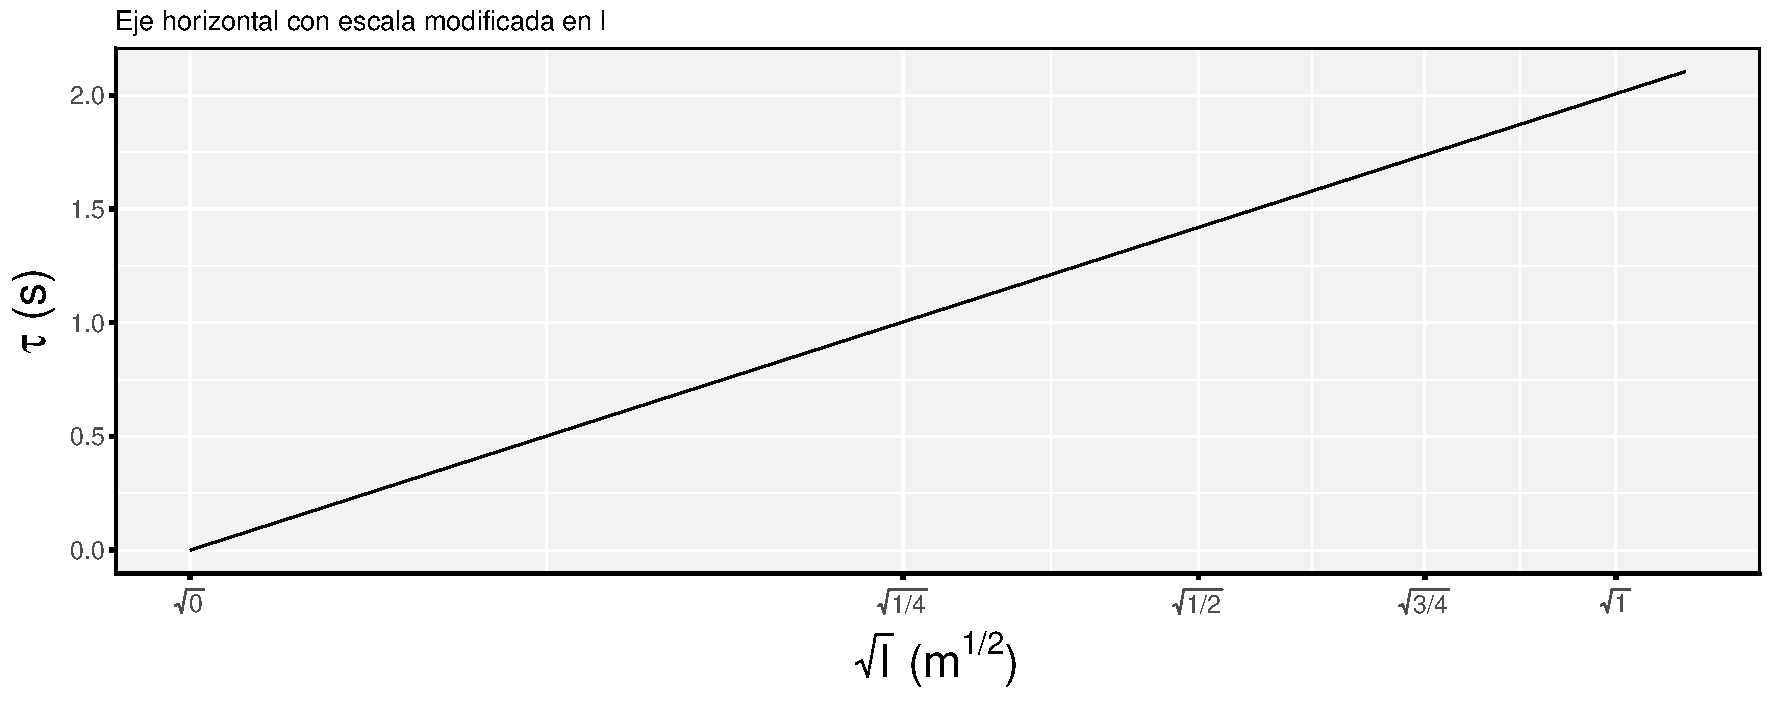
\includegraphics[width=1\linewidth]{./graf/grafrc.pdf}
\vspace*{-2mm}
 \caption{Gráfica del periodo $\tau \, [s]$ \textit{vs.} $\sqrt{l} \, [m^{1/2}]$. Se ve una recta, porque cambiamos la escala del eje horizontal.}  
  \label{gnlin}
\end{figure}


Si miramos detenidamente la ec.\eqref{eltau}, tenemos que:

\begin{itemize}
\item[$\bullet$] La información sobre la \textit{funcionalidad} de $\tau$ se podrá corroborar en el caso en el que los puntos experimentales estén dispuestos sobre una recta, dado que grafiquemos $\tau$ \textit{vs.} $\sqrt{l_{cm}}$. Esto nos permite corroborar si el modelo \textit{funciona}, más allá de si hay sesgos en la estimación de la constante.
\item[$\bullet$] Toda la información sobre $g$ está encapsulada en un parámetro que podemos obtener de los datos, la pendiente de una recta de un ajuste, $A = 2\pi/\sqrt{g}$.
\end{itemize}

Si graficamos $\tau$ \textit{vs.} $\sqrt{l} = x$, deberíamos ver una recta con ordenada al origen \textit{igual a cero} en el caso en el que el modelo dado por la ec.\eqref{tau} se cumpla. Esto presenta una buena manera de sopesar la \textit{funcionalidad} del modelo propuesto, dado que sólo conocemos ajustes lineales de rectas.

Razones pueden haber muchas, pero ya advertimos: la potencia de nuestro análisis de datos está limitada por la falta de opciones de las que disponemos (aunque planeamos ampliar la paleta de opciones). 



\subsubsection*{Ajustando una(s) recta(s) para encontrar \textit{g}}

Hacer un ajuste lineal tiene una infinidad de detalles (si algún día quieren encontrar un parámetro en serio, deberán saberlos), pero nos ayuda a comernos el ruido de todas las medidas. En cierta manera, hacer un ajuste lineal, es encontrar una media muestral en una relación funcional.



\begin{itemize}
\item[\textbf{a)}] Grafique $\overline{\tau} \; vs. \; \sqrt{l_{cm}}$ para todo el curso ¿se ve algo parecido a una recta?
\item[\textbf{b)}] Grafique una recta de referencia $\overline{\tau} = 2 \pi \sqrt{l_{cm}} /\sqrt{g_{RAGA}}$.   
\item[\textbf{c)}] Realice dos ajustes lineales de los datos de todo el curso $\bar{\tau} \; vs. \; \sqrt{l_{cm}}$; el primero, de una recta de la forma $\bar{\tau} = a + b \sqrt{l_{cm}}$, mientras que el segundo, de la forma $\bar{\tau} = b \sqrt{l_{cm}}$. Evalúe cómo se ven las rectas ajustadas con un criterio \textit{visual} (cuál está más cerca). Informe $b \pm SEM_b$ y $R^2$ para ambos ajustes.
\item[g)] De los ajustes anteriores, identifique las pendientes $b$ con los parámetros del modelo de péndulo ideal, obteniendo $g_{ajuste}$
\item[h)] Compare los valores obtenidos de $g$ con $g_{RAGA}$ y discuta posibles problemas y sesgos en los valores obtenidos.
\end{itemize}

\begin{small}
Nota para obtener $g_{ajuste}$:
\end{small}

$$
g_{ajuste} = \frac{2 \pi}{b^2} \;\;\;\;\;\; s_{g\,ajuste} = \frac{2\pi}{b^3} s_b 
$$

\end{document}
